\documentclass[10pt]{article}
\usepackage[utf8]{inputenc}
\usepackage[T1]{fontenc}
\usepackage{amsmath}
\usepackage{amsfonts}
\usepackage{amssymb}
\usepackage{mhchem}
\usepackage{stmaryrd}
\usepackage{graphicx}
\usepackage[export]{adjustbox}
\graphicspath{ {./images/} }

\begin{document}
(ii) Table for determination of diameter \((D)\) of \(\mathrm{r}\)

\texttt{https://cdn.mathpix.com/cropped/a2978538246081aa91be444fc9e0a5aa-1.jpg?height=516&width=1245&top_left_y=666&top_left_x=3}

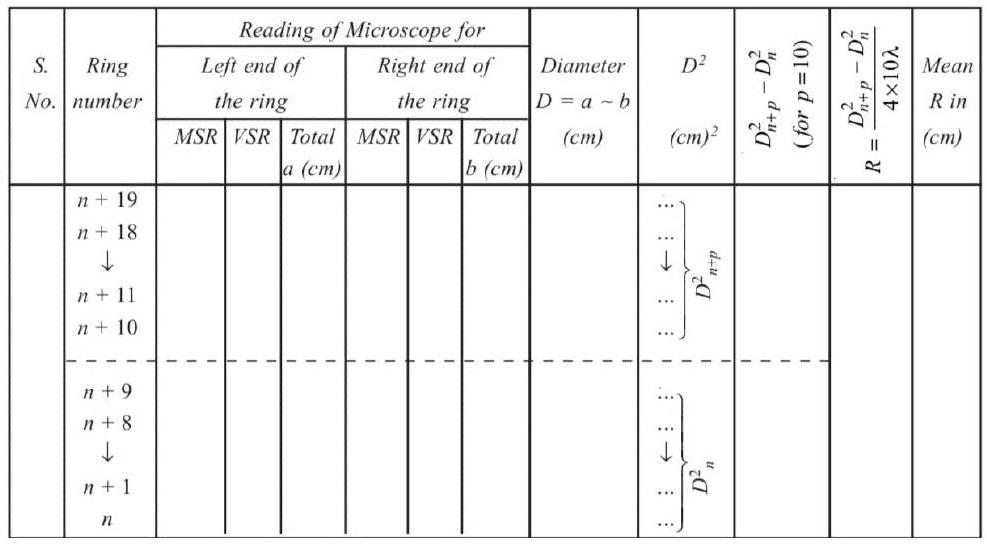
\includegraphics[max width=\textwidth]{a2978538246081aa91be444fc9e0a5aa-2}

Calculations. Using formula EXPERIMENT L-28: To determine the radius of curvature of the lower st plano-convex lens by using Newton's rings apparatus.

Apparatus. Same set up as used in Expt. L27.

Formula. Radius of curvature, \(R=\frac{\text { slope }(m)}{4 \lambda}\)

where, \(\quad l=\) wavelength of light (Sodium lamp, \(l=5893 \AA\) )
\[
m=\text { Slope of line drawn between } D_{n}^{2} \text { and } \mathrm{n}
\]
\[
=\frac{D_{n+p}^{2}-D_{n}^{2}}{p}
\]
Here, \(D_{n+p}\) is the diameter of \((n+p)^{\text {th }}\) ring and \(D_{n}\) that of \(n^{\text {th }}\) ring.

Observations.

(i) Least count vernier of miroscope \(=\ldots . \mathrm{cm}\)

(ii) Table for determination of diameter \((D)\) of rings:

Calculations. Using formula
\[
R=\frac{D_{n+p}^{2}-D_{n}^{2}}{4 \times 10 \lambda}
\]
radius of curvature \(R\) of plano-convex lens can be calculation.

Graph. The value of \(R\) can be determined by plotting a graph taking \(D^{2}\) along \(Y\) -axis and ring number \((n)\) along \(X\) -axis as shown in Fig. \(17.7\).

Two points \(P_{1}\) and \(P_{2}\) are taken on this graph as far apart as possible. The ordinate of \(P_{2}\) is \(P_{2} N_{2}=D_{(n+p)}^{2}\) (say) while the ordinate of \(P_{1}\) is \(P_{1} N_{1}=D_{n}^{2}\) (say).

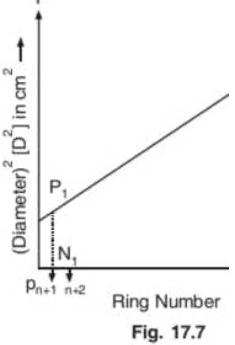
\includegraphics[max width=\textwidth]{a2978538246081aa91be444fc9e0a5aa-4}


\end{document}